% quadrature_decoder - quadrature decoder with or without clock input
% Written in 2016 by <Ahmet Inan> <xdsopl@googlemail.com>
% To the extent possible under law, the author(s) have dedicated all copyright and related and neighboring rights to this software to the public domain worldwide. This software is distributed without any warranty.
% You should have received a copy of the CC0 Public Domain Dedication along with this software. If not, see <http://creativecommons.org/publicdomain/zero/1.0/>.
\documentclass[a4paper]{article}
\usepackage{amsmath}
\usepackage{wrapfig}
\usepackage{gensymb}
\usepackage{hyperref}
\usepackage{fancyvrb}
\usepackage{tikz}
\usepackage{tikz-timing}
\usepackage[bottom]{footmisc}
\usetikzlibrary{circuits.logic.US}
\tikzstyle{branch}=[fill,shape=circle,minimum size=2pt,inner sep=0pt]
\title{Quadrature decoder with or without clock input\\- or -\\How to make a rotary encoder work with\\an FPGA using VHDL}
\author{Ahmet Inan\\\href{mailto:xdsopl@googlemail.com}{\nolinkurl{xdsopl@googlemail.com}}}
\begin{document}
\maketitle
\begin{abstract}
It has been a long time since I played with 74HCT devices to build an 16-Bit-ISA card bus interface.
But times change and you wouldn't do that today having all these nice CPLD (sea of gates) and FPGA (lookup tables) devices and, most important of all, their design synthesis tools.
So I wanted to know, how rotary encoders work, how I could use them with FPGA's and also learn VHDL.
It's gonna be fun, let's go!
\end{abstract}
\begin{wrapfigure}{r}{0.5\textwidth}
\centering
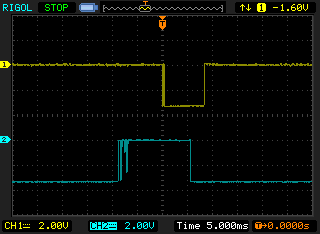
\includegraphics[width=0.5\textwidth]{quadrature_decoder_rigol.png}
\caption{Bounces caused by the mechanical switches of the rotary encoder}
\label{fig:bounces}
\end{wrapfigure}
\section{Contacts of mechanical switches bounce}
Before going to the logic operation side of things, let's first study the signals generated by a mechanical switch-based rotary encoder.
As you can see from the signals captured~\footnote{Image created by Rigol DS1102E oscilloscope and inverted using ImageMagick \emph{convert}.}
by a dual channel oscilloscope in figure~\ref{fig:bounces},
the contacts of the mechanical switches inside of the rotary encoder bounce while switching and create erratic pulses until they finally settle down.
Fortunately, only one of the two signals created by the rotary encoder will ever have those erratic pulses at a time.
So could we apply the things we've learned from debouncing a double throw switch with an SR~latch\footnote{Jack G. Ganssle wrote a very nice article about it: A Guide to Debouncing.}?
Yes, we can!
\newpage
\section{Quadrature signals}
Let's disregard the erratic pulses for a moment so we can focus on the interrelation of the signals created by a rotary encoder, shown in figure~\ref{fig:quadrature}.
\begin{wrapfigure}{l}{0.5\textwidth}
\centering
\begin{tikztimingtable}
& SSS N(A1)SN(A2)SN(A3)SN(A4) SSS SSS SSS N(A5)SN(A6)SN(A7)SN(A8) SSS \\
$A$ & LLL HHL LLL SSS LLL LHH LLL \\
$B$ & LLL LHH LLL SSS LLL HHL LLL \\
& SSS N(B1)SN(B2)SN(B3)SN(B4) SSS SSS SSS N(B5)SN(B6)SN(B7)SN(B8) SSS \\
\extracode
\begin{pgfonlayer}{background}
\node at ($(A1)+(0,0.5)$) {\tiny$1$};
\node at ($(A2)+(0,0.5)$) {\tiny$2$};
\node at ($(A3)+(0,0.5)$) {\tiny$3$};
\node at ($(A4)+(0,0.5)$) {\tiny$4$};
\node at ($(A5)+(0,0.5)$) {\tiny$5$};
\node at ($(A6)+(0,0.5)$) {\tiny$6$};
\node at ($(A7)+(0,0.5)$) {\tiny$7$};
\node at ($(A8)+(0,0.5)$) {\tiny$8$};
\draw[help lines] (A1) -- (B1);
\draw[help lines] (A2) -- (B2);
\draw[help lines] (A3) -- (B3);
\draw[help lines] (A4) -- (B4);
\draw[help lines] (A5) -- (B5);
\draw[help lines] (A6) -- (B6);
\draw[help lines] (A7) -- (B7);
\draw[help lines] (A8) -- (B8);
\end{pgfonlayer}
\end{tikztimingtable}
\caption{Signals in quadrature}
\label{fig:quadrature}
\end{wrapfigure}
On the left you can see waveforms that happen when the wheel of the rotary encoder is turned one step in one direction and one step in the opposite direction is what you see on the right side.
These signals are said to be \emph{in quadrature}~\footnote{\href{https://en.wikipedia.org/wiki/In-phase_and_quadrature_components}{Wikipedia on: In-phase and quadrature components.}} as their relation is that they are orthogonal to each other or in simpler terms, $90\degree$ out of phase.
We can also gather that there are only four signal level constellations we have to consider and creating the signals to be debounced by our trusty SR~latches is now easy:
\begin{align}
1\mbox{--}2, 7\mbox{--}8 &:& A = H &\land B = L &\implies& E \gets A \land \neg B\\
2\mbox{--}3, 6\mbox{--}7 &:& A = H &\land B = H &\implies& C \gets A \land B\\
3\mbox{--}4, 5\mbox{--}6 &:& A = L &\land B = H &\implies& F \gets B \land \neg A\\
    else &:& A = L &\land B = L &\implies& D \gets \neg (A \lor B)
\end{align}
\section{Design with logic gates}
\begin{wrapfigure}{r}{0.5\textwidth}
\centering
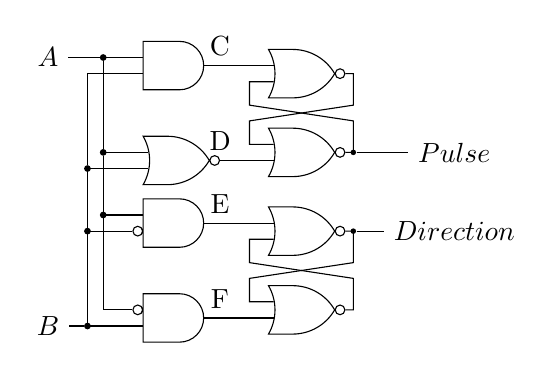
\begin{tikzpicture}[circuit logic US]
\node[nor gate, draw, inputs=nn] at (3,0) (Nor2) {};
\node[nor gate, draw, inputs=nn] at (3,1) (Nor3) {};
\node[nor gate, draw, inputs=nn] at (3,2) (Nor4) {};
\node[nor gate, draw, inputs=nn] at (3,3) (Nor5) {};
\node[and gate, draw, inputs=ni] at ($(Nor3.input 1)+(-1.3,0)$) (And1) {};
\node[and gate, draw, inputs=in] at ($(Nor2.input 2)+(-1.3,0)$) (And2) {};
\node[and gate, draw, inputs=nn] at ($(Nor5.input 1)+(-1.3,0)$) (And3) {};
\node[nor gate, draw, inputs=nn] at ($(Nor4.input 2)+(-1.3,0)$) (Nor1) {};
\node[branch, draw] at ($(And3.input 1)+(-0.5,0)$) (A1) {};
\node[branch, draw] at ($(A1 |- Nor1.input 1)$) (A2) {};
\node[branch, draw] at ($(A1 |- And1.input 1)$) (A3) {};
\node[branch, draw] at ($(And2.input 2)+(-0.7,0)$) (B1) {};
\node[branch, draw] at ($(B1 |- And1.input 2)$) (B2) {};
\node[branch, draw] at ($(B1 |- Nor1.input 2)$) (B3) {};
\node (A) at ($(A1)+(-0.7,0)$) {$A$};
\node (B) at ($(B1)+(-0.5,0)$) {$B$};
\node (P) at ($(Nor4)+(2,0)$) {$Pulse$};
\node (D) at ($(Nor3)+(2,0)$) {$Direction$};
\draw (A) -- (A1);
\draw (B) -- (B1);
\draw (A1) -- (A2);
\draw (A2) -- (A3);
\draw (B1) -- (B2);
\draw (B2) -- (B3);
\draw (A3) |- (And1.input 1);
\draw (B2) |- (And1.input 2);
\draw (A3) |- (And2.input 1);
\draw (B1) |- (And2.input 2);
\draw (A1) |- (And3.input 1);
\draw (B3) |- (And3.input 2);
\draw (A2) |- (Nor1.input 1);
\draw (B3) |- (Nor1.input 2);
\draw (And1.output) -- +(0.2,0) node[above]{E} -- (Nor3.input 1);
\draw (And2.output) -- +(0.2,0) node[above]{F} -- (Nor2.input 2);
\draw (Nor3.output) -| node[branch] (D1) {} +(0.1,-0.4) -- ($(Nor2)+(-0.6,+0.4)$) |- (Nor2.input 1);
\draw (Nor2.output) -| +(0.1,0.4) -- ($(Nor3)+(-0.6,-0.4)$) |- (Nor3.input 2);
\draw (D1) -- (D);
\draw (And3.output) -- +(0.2,0) node[above]{C} -- (Nor5.input 1);
\draw (Nor1.output) -- +(0,0) node[above]{D} -- (Nor4.input 2);
\draw (Nor5.output) -| +(0.1,-0.4) -- ($(Nor4)+(-0.6,+0.4)$) |- (Nor4.input 1);
\draw (Nor4.output) -| node[branch] (P1) {} +(0.1,0.4) -- ($(Nor5)+(-0.6,-0.4)$) |- (Nor5.input 2);
\draw (P1) -- (P);
\end{tikzpicture}
\caption{Logic gate circuit}
\label{fig:asyn_logic}
\end{wrapfigure}
Putting those new signals $C$--$F$ to good use and designing a circuit made from logic gates should lead us to something like shown in figure~\ref{fig:asyn_logic}.
Before immediately jumping to build the circuit in hardware (now that you have the circuit) please be aware that the signals shown in figure~\ref{fig:quadrature} are active high signals.
With TTL logic you usually use pull-up resistors~\footnote{\href{https://en.wikipedia.org/wiki/Pull-up_resistor}{Wikipedia on: Pull-up resistor.}} with mechanical switches and thus have active low signals.
The reason being that it needs a much higher current when driving an TTL input low than high.
With CMOS logic it doesn't matter: you can exchange pull-up with pull-down resistors for the mechanical switches, therefore inverting the signal with no problems.
Using active low signals with this circuit will make it work unreliable and you should redesign the circuit if you intend to go that way (bonus points to those who do).
So is it really gonna work if we build it? Let's~find~out!
\newpage
\section{Circuit analysis}
\begin{wrapfigure}{l}{0.5\textwidth}
\centering
\begin{tikztimingtable}
$A$         & LLL N(A1)HHN(A2)L LLL LN(A3)HHN(A4) LLL \\
$B$         & LLL LN(B1)HHN(B2) LLL N(B3)HHN(B4)L LLL \\
$C$         & LLL LN(C1)HN(C2)L LLL LN(C3)HN(C4)L LLL \\
$D$         & HHH N(D1)LLLN(D2) HHH N(D3)LLLN(D4) HHH \\
$E$         & LLL N(E1)HN(E2)LL LLL LLN(E3)HN(E4) LLL \\
$F$         & LLL LLN(F1)HN(F2) LLL N(F3)HN(F4)LL LLL \\
$Pulse$     & LLL LN(P1)HHN(P2) LLL LN(P3)HHN(P4) LLL \\
$Direction$ & LLL LLN(D1)H HHH HHN(D2)L LLL \\
\extracode
\begin{pgfonlayer}{background}
\draw[help lines] (A1) -- (E1);
\draw[help lines] (A2) -- (D1);
\draw[help lines] (A3) -- (P3);
\draw[help lines] (A4) -- (P4);
\draw[help lines] (B1) -- (P1);
\draw[help lines] (B2) -- (P2);
\draw[help lines] (B3) -- (F3);
\draw[help lines] (B4) -- (D2);
\end{pgfonlayer}
\end{tikztimingtable}
\caption{Clean waveforms}
\label{fig:asyn_wave}
\end{wrapfigure}
Carefully analysing the waveforms of the signals $C$--$F$, $Pulse$ and $Direction$ created by our circuit when stimulated by the clean signals $A$ and $B$ might look like in figure~\ref{fig:asyn_wave}.
We can see, that the high levels of the signal pairs $C, D$ and $E, F$ do not overlap.
This is important for the SR latch to work correctly, as the state when both inputs are high would cause a race condition~\footnote{\href{https://en.wikibooks.org/wiki/Digital_Circuits/Latches}{Wikibooks on: Digital Circuits/Latches}}, leading to undefined behavior.
Even the signals $Pulse$ and $Direction$ look good: $Direction$ stays steady while $Pulse$ is going from low to high.
Those are exactly the signals we can use with rising edge-triggered devices.
Setup and hold times shouldn't be an issue either, as the electronic devices we are going to use are many orders of magnitude faster than the signals created by our mechanical rotary switches.
So let's build it. With VHDL!
\section{Design with VHDL}
\begin{wrapfigure}{r}{0.5\textwidth}
\centering
\begin{BVerbatim}
c <= a and b;
d <= a nor b;
e <= a and not b;
f <= b and not a;
dir <= dir_n nor e;
dir_n <= dir nor f;
pul <= pul_n nor d;
pul_n <= pul nor c;
pulse <= pul;
direction <= dir;
\end{BVerbatim}
\caption{VHDL code}
\label{fig:asyn_vhdl}
\end{wrapfigure}
Signals $A$ and $B$ are the inputs we have and need to create the signals for the outputs $Pulse$ and $Direction$ of our circuit.
Keeping in mind that VHDL statements run concurrently, we can easily write our circuit from figure~\ref{fig:asyn_logic} down like in figure~\ref{fig:asyn_vhdl}
But wait a minute, aren't we creating race conditions here already?
Nope, and here's why: VHDL uses something called the \emph{delta cycle algorithm}\footnote{Jan Decaluwe wrote a very nice article about it: VHDL's crown jewel.} to simulate the circuit.
In short: Signal assignments in VHDL get their value updated in the next delta cycle, just like a physical logic gate would deliver its new resulting output value after some time has past when stimulated by new input values.
Okay, but why are we using signals $A$ and $B$ directly in our VHDL circuit but $Pulse$ and $Direction$ not?
If you look closer, $A$ and $B$ are used exclusively as inputs whereas the signal pairs $dir,dir\_n$ and $pul,pul\_n$ are used as inputs and outputs at the same time.
With the last two simple signal assignments we can keep the signals $Pulse$ and $Direction$ strictly as outputs.
Can we please see the circuit in action now? Quick, to the testbench!
\newpage
\section{Testbench}
What I didn't realise at first while working with VHDL was that having a testbench is such an awesome concept.
We can actually create a virtual environment where we can test our design in isolation and do all kinds of nasty stimulations we can think of to it, without ever worrying about the magic smoke to come out.
Even nicer is the fact, that there are free and open source tools like GHDL~\footnote{\url{http://ghdl.free.fr/}} for VHDL simulation and GTKWave~\footnote{\url{http://gtkwave.sourceforge.net/}} for waveform visualization.
Those two are the only tools you will ever need if you want to learn to code in VHDL.
The result of running a testbench simulation on the VHDL code from figure~\ref{fig:asyn_vhdl} in GHDL and visualized in GTKWave would look like in figure~\ref{fig:asyn_wave}.
\begin{figure}[h]
\centering
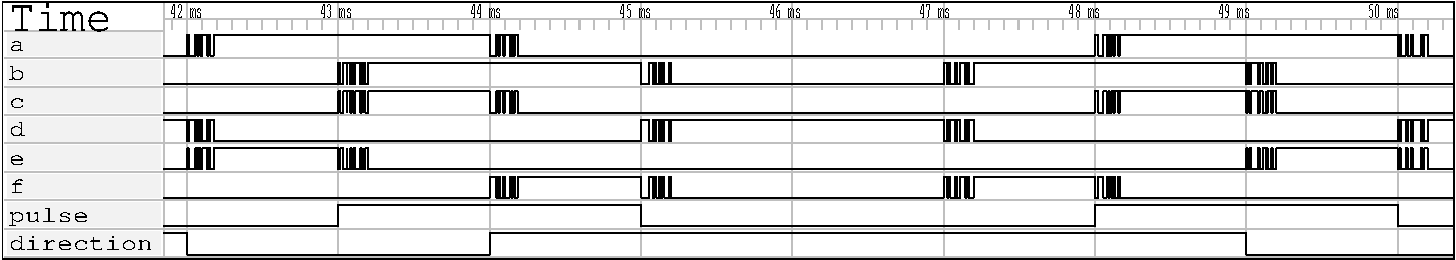
\includegraphics[width=\textwidth]{asynchronous_quadrature_decoder_gtkwave.pdf}
\caption{Waveforms of asynchronous design}
\label{fig:asyn_wave}
\end{figure}
As you can see, we are even able to simulate the contact bounces in a testbench!
Signals $A$--$F$ have the erratic pulses but behold, the $Pulse$ and $Direction$ signals are properly debounced by the SR latches.
If you want to run this testbench on your own, this is the place where you should stop reading and have fun with the VHDL code on my GitHub page: \url{https://github.com/xdsopl/vhdl}
\\Had fun? Thought so. Let's continue with the hardware.
\section{Which FPGA vendor}
For my FPGA experiments I ordered an Altera MAX10 devkit~\footnote{\href{https://www.altera.com/products/boards_and_kits/dev-kits/altera/kit-max-10-evaluation.html}{Altera MAX 10 FPGA Evaluation Kit EK-10M08E144ES/P}} on Digi-Key~\footnote{\href{http://www.digikey.de/short/3pd4ch}{Digi-Key Part Number: 544-3042-ND}}.
That's why I'm going to continue with the results and screenshots~\footnote{Used "print to PDF" and edited in Inkscape} made from Altera's free Quartus~Prime~Lite~Edition~\footnote{\url{http://dl.altera.com/?edition=lite}} design software.
Don't forget to order an download cable with the above devkit, as it has no onboard programmer.
I ended up ordering the cheaper USB Blaster clone from Terasic on Digi-Key~\footnote{\href{http://www.digikey.de/short/3pd4j9}{Digi-Key Part Number: P0302-ND}} which also works with the software from Altera.
The only thing I couldn't understand was the lack of galvanic isolation for a simple device of such high price.
So be careful when poking around for differential signals with your oscilloscope\footnote{Dave Jones made a very nice video about it: \href{https://youtu.be/xaELqAo4kkQ}{How NOT To Blow Up Your Oscilloscope!}}.
With the decision over which hardware to choose cleared out of the way, let's continue and use Quartus to synthesize our VHDL design.
\newpage
\section{Hardware synthesis}
The VHDL code from figure~\ref{fig:asyn_vhdl} compiled in Quartus and viewed in it's RTL~Viewer looks like in figure~\ref{fig:asyn_rtl}.
\begin{figure}[h]
\centering
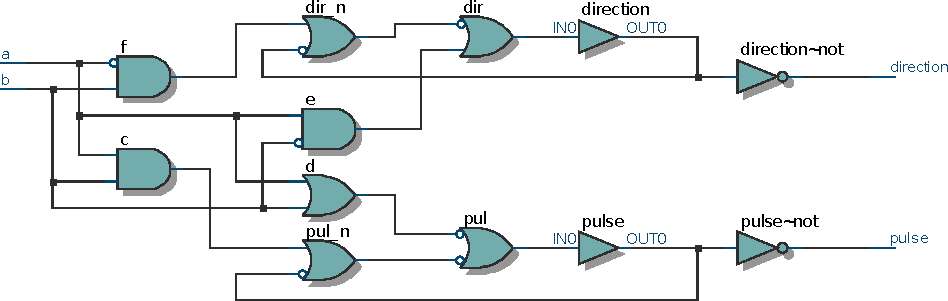
\includegraphics[width=\textwidth]{asynchronous_quadrature_decoder_quartus_rtl.pdf}
\caption{RTL view of our design}
\label{fig:asyn_rtl}
\end{figure}
It might look a little odd but it is essentially the same circuit as in figure~\ref{fig:asyn_logic}
But we are more interested about the configuration that will later land on the FPGA.
That's where the Technology Map Viewer comes into play and our design looks like in figure~\ref{fig:asyn_map}
\begin{figure}[h]
\centering
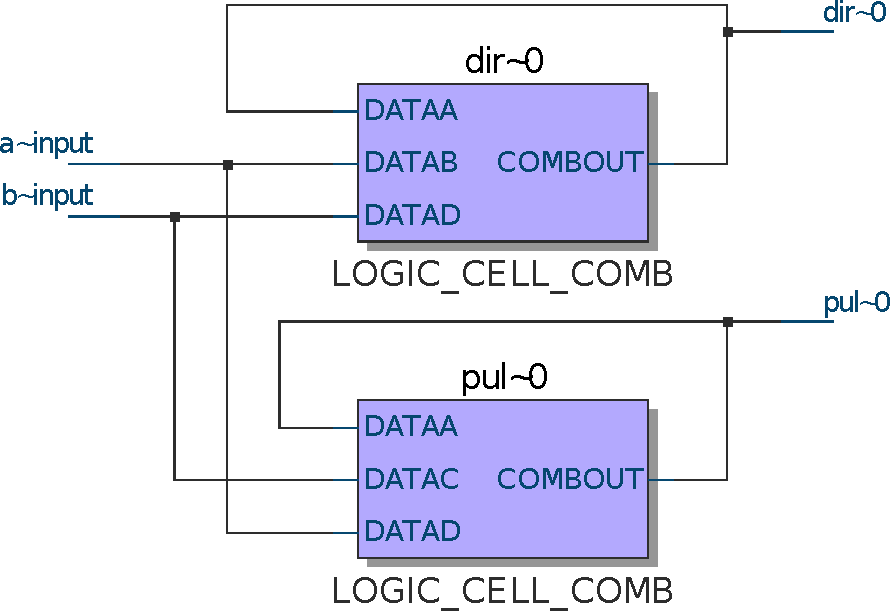
\includegraphics[width=0.5\textwidth]{asynchronous_quadrature_decoder_quartus_map.pdf}
\caption{Reduced to two combinational loops}
\label{fig:asyn_map}
\end{figure}
Wow, just two lookup tables! And it works, too!
It still looks to good to be true and indeed this configuration harbours hidden dangers as we can see some hints from Quartus shown in figure~\ref{fig:warning}.
\begin{figure}[h]
\centering
\begin{BVerbatim}
Warning: Found combinational loop of 2 nodes
Warning (332126): Node "decoder_inst|pul~0|dataa"
Warning (332126): Node "decoder_inst|pul~0|combout"
Warning: Found combinational loop of 2 nodes
Warning (332126): Node "decoder_inst|dir~0|dataa"
Warning (332126): Node "decoder_inst|dir~0|combout"
\end{BVerbatim}
\caption{Combinational loop warning}
\label{fig:warning}
\end{figure}
The problem lies within the feedback of $COMBOUT$ to $DATAA$.
But it works fine, I tried it, so why the fuss? Let's look at how lookup tables work.
\newpage
\section{Lookup tables}
\begin{wrapfigure}{r}{0.5\textwidth}
\centering
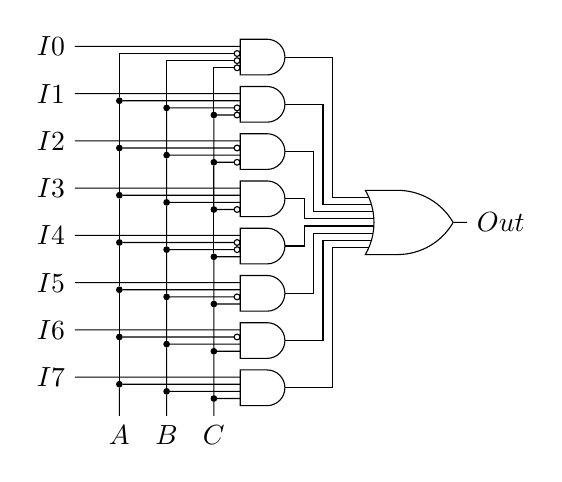
\begin{tikzpicture}[scale=0.6, circuit logic US]
\node (A) at (1,0) {$A$};
\node (B) at (2,0) {$B$};
\node (C) at (3,0) {$C$};
\node[and gate, draw, inputs=niii] at (4,8) (And0) {};
\node[and gate, draw, inputs=nnii] at (4,7) (And1) {};
\node[and gate, draw, inputs=nini] at (4,6) (And2) {};
\node[and gate, draw, inputs=nnni] at (4,5) (And3) {};
\node[and gate, draw, inputs=niin] at (4,4) (And4) {};
\node[and gate, draw, inputs=nnin] at (4,3) (And5) {};
\node[and gate, draw, inputs=ninn] at (4,2) (And6) {};
\node[and gate, draw, inputs=nnnn] at (4,1) (And7) {};
\node[or gate, draw, inputs=nnnnnnnn] at (7,4.5) (Or0) {};
\node (O) at ($(Or0.output)+(1,0)$) {$Out$};
\node (I0) at ($(And0.input 1)+(-4,0)$) {$I0$};
\node (I1) at ($(And1.input 1)+(-4,0)$) {$I1$};
\node (I2) at ($(And2.input 1)+(-4,0)$) {$I2$};
\node (I3) at ($(And3.input 1)+(-4,0)$) {$I3$};
\node (I4) at ($(And4.input 1)+(-4,0)$) {$I4$};
\node (I5) at ($(And5.input 1)+(-4,0)$) {$I5$};
\node (I6) at ($(And6.input 1)+(-4,0)$) {$I6$};
\node (I7) at ($(And7.input 1)+(-4,0)$) {$I7$};
\node[branch, draw] at ($(And1.input 2 -| A)$) (A1) {};
\node[branch, draw] at ($(And1.input 3 -| B)$) (B1) {};
\node[branch, draw] at ($(And1.input 4 -| C)$) (C1) {};
\node[branch, draw] at ($(And2.input 2 -| A)$) (A2) {};
\node[branch, draw] at ($(And2.input 3 -| B)$) (B2) {};
\node[branch, draw] at ($(And2.input 4 -| C)$) (C2) {};
\node[branch, draw] at ($(And3.input 2 -| A)$) (A3) {};
\node[branch, draw] at ($(And3.input 3 -| B)$) (B3) {};
\node[branch, draw] at ($(And3.input 4 -| C)$) (C3) {};
\node[branch, draw] at ($(And4.input 2 -| A)$) (A4) {};
\node[branch, draw] at ($(And4.input 3 -| B)$) (B4) {};
\node[branch, draw] at ($(And4.input 4 -| C)$) (C4) {};
\node[branch, draw] at ($(And5.input 2 -| A)$) (A5) {};
\node[branch, draw] at ($(And5.input 3 -| B)$) (B5) {};
\node[branch, draw] at ($(And5.input 4 -| C)$) (C5) {};
\node[branch, draw] at ($(And6.input 2 -| A)$) (A6) {};
\node[branch, draw] at ($(And6.input 3 -| B)$) (B6) {};
\node[branch, draw] at ($(And6.input 4 -| C)$) (C6) {};
\node[branch, draw] at ($(And7.input 2 -| A)$) (A7) {};
\node[branch, draw] at ($(And7.input 3 -| B)$) (B7) {};
\node[branch, draw] at ($(And7.input 4 -| C)$) (C7) {};
\draw (I0) -- (And0.input 1);
\draw (I1) -- (And1.input 1);
\draw (I2) -- (And2.input 1);
\draw (I3) -- (And3.input 1);
\draw (I4) -- (And4.input 1);
\draw (I5) -- (And5.input 1);
\draw (I6) -- (And6.input 1);
\draw (I7) -- (And7.input 1);
\draw (A1) |- (And0.input 2);
\draw (B1) |- (And0.input 3);
\draw (C1) |- (And0.input 4);
\draw (A1) -- (And1.input 2);
\draw (B1) -- (And1.input 3);
\draw (C1) -- (And1.input 4);
\draw (A2) -- (And2.input 2);
\draw (B2) -- (And2.input 3);
\draw (C2) -- (And2.input 4);
\draw (A3) -- (And3.input 2);
\draw (B3) -- (And3.input 3);
\draw (C3) -- (And3.input 4);
\draw (A4) -- (And4.input 2);
\draw (B4) -- (And4.input 3);
\draw (C4) -- (And4.input 4);
\draw (A5) -- (And5.input 2);
\draw (B5) -- (And5.input 3);
\draw (C5) -- (And5.input 4);
\draw (A6) -- (And6.input 2);
\draw (B6) -- (And6.input 3);
\draw (C6) -- (And6.input 4);
\draw (A7) -- (And7.input 2);
\draw (B7) -- (And7.input 3);
\draw (C7) -- (And7.input 4);
\draw (A) -- (A7);
\draw (B) -- (B7);
\draw (C) -- (C7);
\draw (A1) -- (A2);
\draw (B1) -- (B2);
\draw (C1) -- (C2);
\draw (A2) -- (A3);
\draw (B2) -- (B3);
\draw (C2) -- (C3);
\draw (A3) -- (A4);
\draw (B3) -- (B4);
\draw (C2) -- (C4);
\draw (A4) -- (A5);
\draw (B4) -- (B5);
\draw (C4) -- (C5);
\draw (A5) -- (A6);
\draw (B5) -- (B6);
\draw (C5) -- (C6);
\draw (A6) -- (A7);
\draw (B6) -- (B7);
\draw (C6) -- (C7);
\draw (And0.output) -- +(1,0) |- (Or0.input 1);
\draw (And1.output) -- +(0.8,0) |- (Or0.input 2);
\draw (And2.output) -- +(0.6,0) |- (Or0.input 3);
\draw (And3.output) -- +(0.4,0) |- (Or0.input 4);
\draw (And4.output) -- +(0.4,0) |- (Or0.input 5);
\draw (And5.output) -- +(0.6,0) |- (Or0.input 6);
\draw (And6.output) -- +(0.8,0) |- (Or0.input 7);
\draw (And7.output) -- +(1,0) |- (Or0.input 8);
\draw (Or0.output) -- (O);
\end{tikzpicture}
\caption{Lookup table logic circuit}
\label{fig:lut_logic}
\end{wrapfigure}
There are actually a lot of different implementation designs for lookup tables solving one or another problem depending on their use case and constraints.
A possible implementation using logic gates is shown in figure~\ref{fig:lut_logic}.
As you can see, changing the value of a single signal like for example $A$ would stimulate almost every single logic gate in parallel and therefore a lot of transistors.
Not every transistor is born equal on the same die: some of them will switch faster whereas others will be weaker, etc.
So we have the problem, that not every signal constellation on the inputs $A$--$C$ will result in the simultaneous switching of all transistors and thus we have overlapping transitions on the outputs of the logic gates, causing glitches.
Some FPGA vendors guarantee~\footnote{You have to wade through forum posts to get something from officials :(} that their LUT implementation won't glitch on a value change of a single input or if all value permutations of the signals involved would result in the same output.
Even if we would have an implementation that would guarantee a glitch free operation on multiple signals changing at once, we would still experience glitches, as it can't be guaranteed that all input signals will change their value simultaneously.
In figure~\ref{fig:glitch} we see the waveforms and a glitch happening to a guaranteed glitch free operating lookup table with the constant value signals $I0$--$I7$ and beeing stimulated by the signals $A$--$C$.
\begin{figure}[h]
\centering
\begin{tikztimingtable}[xscale=0.22,yscale=0.7]
$I0$  & 200H \\
$I1$  & 200L \\
$I2$  & 200H \\
$I3$  & 200L \\
$I4$  & 200L \\
$I5$  & 200L \\
$I6$  & 200L \\
$I7$  & 200L \\
$A$   & 25L 25H N(A1) 25L 25H N(A2) 25L 25H 25L 25H \\
$B$   & 51L 50H N(B1) 50L 49H \\
$C$   & 102L 98H \\
$Out$ & 25H 25L N(O1)25H 25L N(O2)HN(O3) 24L 25L 25L 25L \\
\extracode
\begin{pgfonlayer}{background}
\draw[help lines] (A1) -- (O1);
\draw[help lines] (A2) -- (O2);
\draw[help lines] (B1) -- (O3);
\end{pgfonlayer}
\end{tikztimingtable}
\caption{Glitch on $Out$ when multiple inputs change at almost the same time}
\label{fig:glitch}
\end{figure}
Looking closer at the edges of the signals $A$--$C$ you can see, that they do not arrive at the same time: $A$ comes before $B$ and $B$ comes before $C$.
That little delay causes a glitch that could easily ruin your day.
Depending on the load of the outputs and routing of the signals, such unequal delays are hard to avoid and should be dealt with using more practical methods.
Enter the world of synchronous designs.
\newpage
\section{Register-transfer level}
Fixing the glitch is so easy, that it is almost boring: use an externally clocked register in the feedback loop!
Even the VHDL code get's simpler as you can see in figure~\ref{fig:syn_vhdl}.
\begin{figure}[h]
\centering
\begin{BVerbatim}
c <= a xor b;
dir <= b when rising_edge(clock) and c = '1' else dir;
pul <= a when rising_edge(clock) and c = '0' else pul;
pulse <= pul;
direction <= dir;
\end{BVerbatim}
\caption{VHDL code of synchronous design}
\label{fig:syn_vhdl}
\end{figure}
We sample $A$ or $B$ on the rising edge of our external $Clock$ signal, which should be clocked slower than the output stabilization time of the lookup tables inside the FPGA but at least two times faster~\footnote{See Nyquist limit.} than the shortest stable~\footnote{Not accounting for the contact bounce pulses.} pulse seen on our signal $C$.
Putting the synchronous design in a testbench gives us the waveforms shown in figure~\ref{fig:syn_wave}.
\begin{figure}[h]
\centering
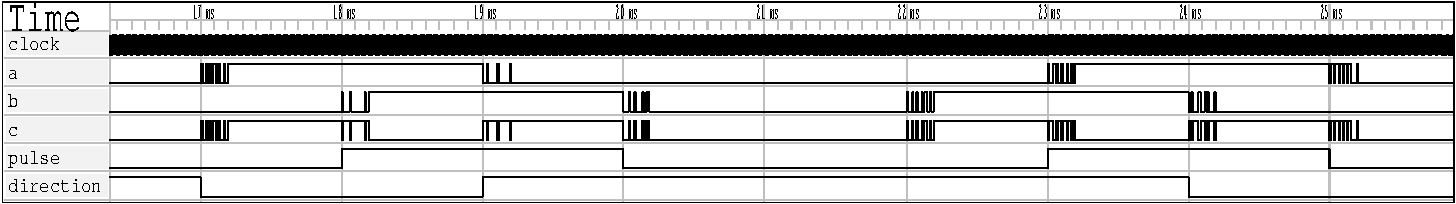
\includegraphics[width=\textwidth]{quadrature_decoder_gtkwave.pdf}
\caption{Waveforms of synchronous design}
\label{fig:syn_wave}
\end{figure}
Properly debounced signals $Pulse$ and $Direction$ and exactly with the timing needed for edge triggered devices!
For completeness sake, let's also look at the quite boring RTL view in figure~\ref{fig:syn_rtl}.
Just one XOR gate and two D-type flip-flops with clock enable input.
\begin{figure}[h]
\centering
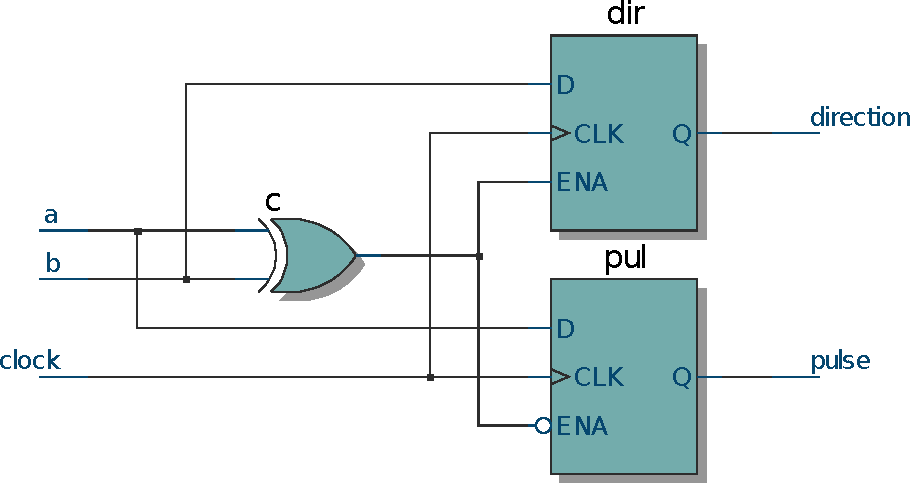
\includegraphics[width=0.5\textwidth]{quadrature_decoder_quartus_rtl.pdf}
\caption{RTL view of synchronous design}
\label{fig:syn_rtl}
\end{figure}
Let's finish up here quickly by looking at the technology map view in figure~\ref{fig:syn_map}.
\begin{figure}[h]
\centering
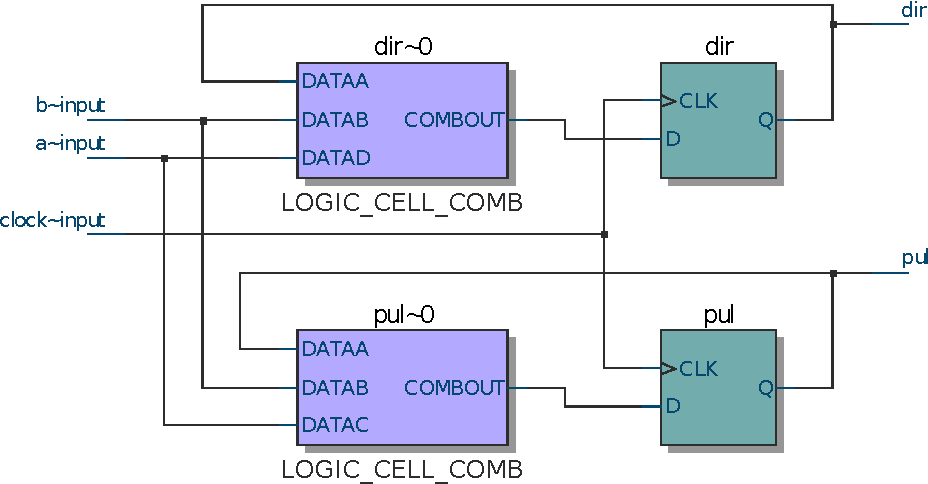
\includegraphics[width=0.7\textwidth]{quadrature_decoder_quartus_map.pdf}
\caption{Technology map view of synchronous design}
\label{fig:syn_map}
\end{figure}
\end{document}
